\documentclass[handout]{beamer}


\usepackage[english]{babel}  
\usepackage[utf8]{inputenc}  
\usepackage[T1]{fontenc}       
\usepackage{amsmath}
\usepackage{amssymb}
\usepackage{dsfont}
\usepackage{graphicx}
\usepackage{float}
\usepackage{stmaryrd}
\usepackage{listings}
\usepackage{color}
\usepackage{amsthm}
\usepackage{subcaption}
\usepackage{tikz}

\usepackage{cite}
\usepackage{amsfonts}
\usepackage{algorithm}
\usepackage{algpseudocode}
\usepackage{algorithmicx}

%\usetheme{Warsaw}
\usetheme{Paloalto}

\AtBeginSection[]
{
  \begin{frame}{Table of Contents}
  \tableofcontents[currentsection, hideothersubsections, pausesubsections]
  \end{frame} 
}


\title{Apprentissage profond, réseau de neurones, etc.}
\author{Antoine BIARD \& Vincent BODIN}


\begin{document}

\renewcommand{\contentsname}{Sommaire}


\begin{frame}[allowframebreaks]
\titlepage
\end{frame}

\section*{Introduction}

\begin{frame}{Introduction}
\begin{itemize}
\item Souvent, l'extraction d'une représentation repose sur une connaissance \emph{a priori} des données ;

\item quantité de données différentes pose la question de la généralité de cette méthode ;

\item volonté d'extraire - de manière non-supervisée - une représentation qui agrège l'information ; 

\item méthode profonde semblent produire ce résultat avec des représentations de plus en plus abstraites.
\end{itemize}
\end{frame}



\section{Revue élémentaire des méthodes de deep learning}

\subsection{Réseau de neurones}

\begin{frame}{Réseau de neurones}
\begin{figure}[ht!]
\centering
\begin{tabular}{cc}
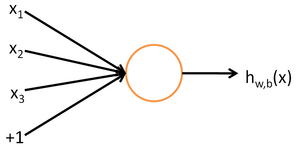
\includegraphics[width = .4\columnwidth]{../fig/SingleNeuron.png} &
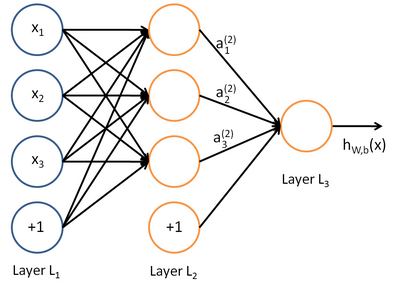
\includegraphics[width = .4\columnwidth]{../fig/Network331.png} 
\end{tabular}
\caption{(gauche) Un neurone avec trois entrées $(x_1,x_2,x_3)$ et un \emph{offset} ; (droite) un réseau de neurones de taille $(3,3,1)$ avec des \emph{offset} aux deux premières couches.}
\label{fig1}
\end{figure}
\begin{block}{Sortie d'un neurone simple}
\begin{equation}
h_{w,b}(x)=\sigma(w^Tx)=\sigma\left(\sum_{i=1}^p w_i x_i + b\right)
\end{equation}
\end{block}
\end{frame}



\subsection{Multilayer Perceptron (MLP)}

\begin{frame}{Multilayer Perceptron (MLP)}
\begin{figure}[ht!]
\centering
\begin{tabular}{cc}
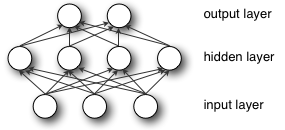
\includegraphics[width = .5\columnwidth]{../fig/mlp} &
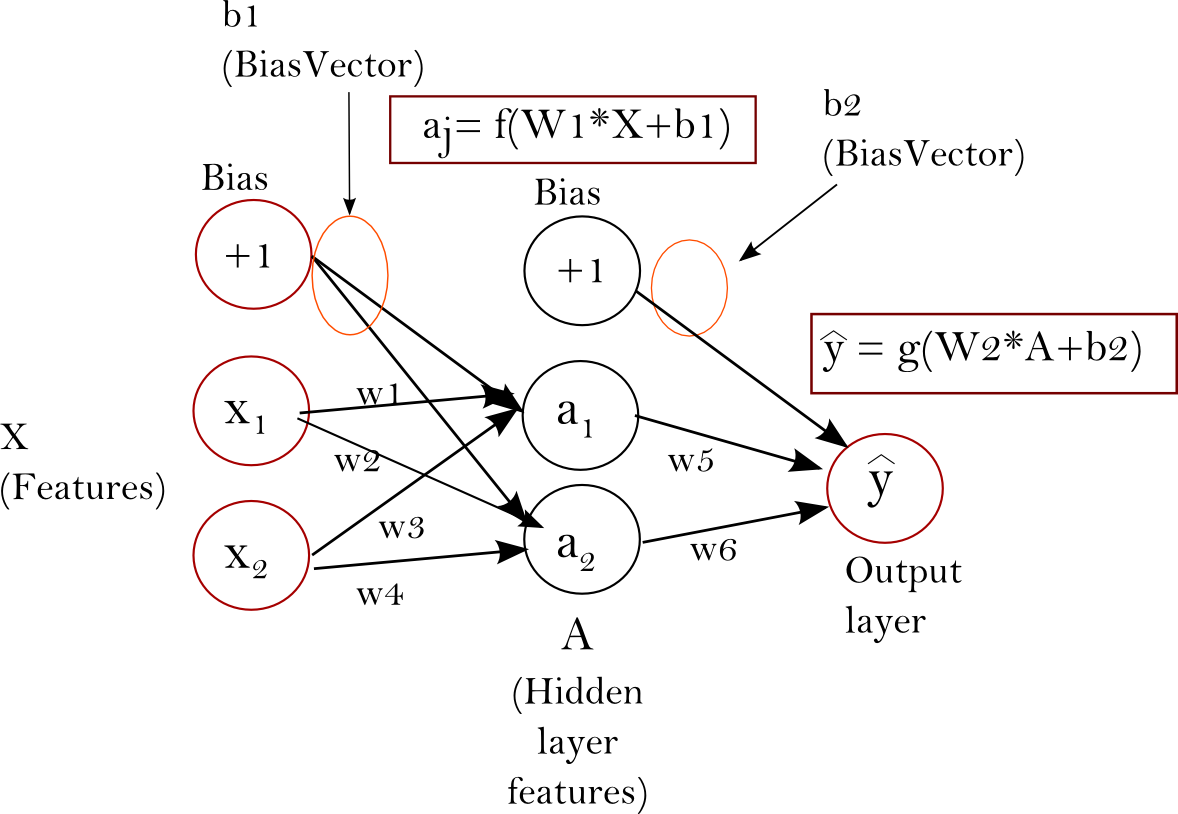
\includegraphics[width = .5\columnwidth]{../fig/backprop_notation.png} 
\end{tabular}
\caption{(gauche) Un MLP avec une seule couche de variables cachées ; (droite) structure de MLP avec l'ajout de biais et les poids.}
\label{fig2}
\end{figure}
\end{frame}



\begin{frame}{Multilayer Perceptron (MLP)}
\begin{block}{Sortie d'un nœud}
\begin{equation}
s(x) = \sigma(Wx + b)
\end{equation}
\end{block}
Le MLP diffère par la manière d'entraîner :
\begin{description}
\item[Forward pass. ]On part des variables visibles $v$ et on remonte le graphe avec les poids de la structure.
\item[Backpropagation. ]Chemin inverse en descendant le graphe et en comptabilisant les erreurs commises, mise à jour les poids.
\end{description}
\end{frame}



\subsection{Restricted Boltzmann Machine (RBM)}

\begin{frame}{Machine de Boltzmann}
\begin{figure}[ht!]
\centering
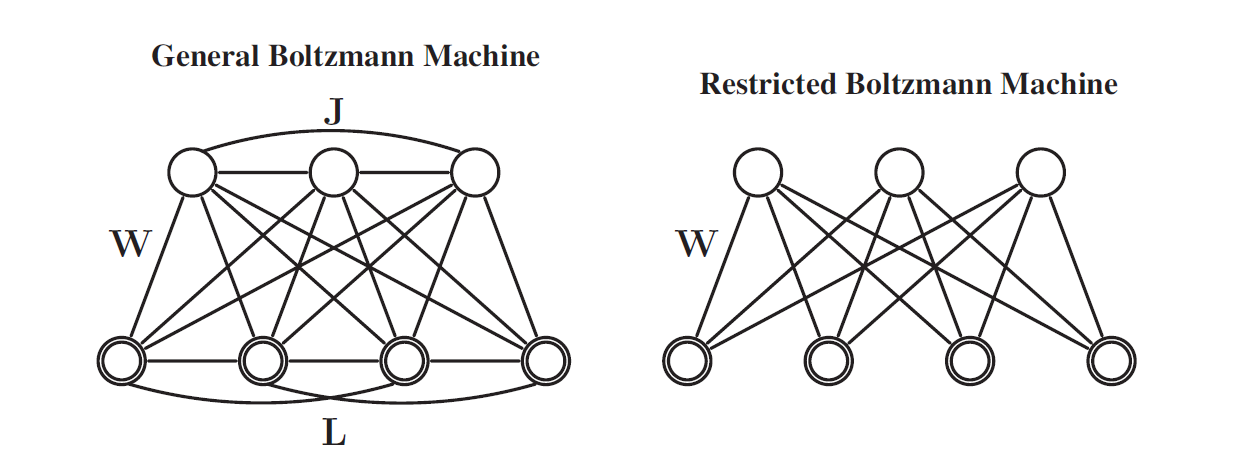
\includegraphics[width = \columnwidth]{../fig/boltzmann_machine.png}
\caption{(gauche) Machine de Boltzmann générale ; (droite) RBM.}
\label{fig3}
\end{figure}
\begin{block}{Énergie}
\begin{equation}
E(v,h ; \theta) = -v^TWh - \frac{1}{2}v^TLv - \frac{1}{2}h^T Jh
\end{equation}
(pas de terme de biais ici)
\end{block}
\end{frame}

\begin{frame}{Restricted Boltzmann Machine}
\begin{itemize}
\item La factorisation dans le graphe donne : 
\begin{equation}
\begin{array}{rll}
p(h|v) & = & \displaystyle \prod_{i} p(h_i|x) \\
p(v|h) & = & \displaystyle \prod_{j} p(x_j|h)
\end{array}
\end{equation}

\item Les probabilités conditionnelles valent : 
\begin{equation}
\begin{array}{rll}
p(h_i = 1 |v ) & = & \displaystyle \sigma\left(\sum_j W_{ji}x_j + d_i\right) \\
p(x_j = 1 |h ) & = & \displaystyle \sigma\left(\sum_i W_{ji}h_i + b_j\right)
\end{array}
\end{equation}
\end{itemize}
\end{frame}




\subsection{Deep Belief Networks (DBN)}

\begin{frame}{Deep Belief Networks (DBN)}
\begin{figure}[ht!]
\centering
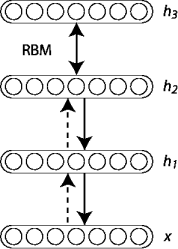
\includegraphics[width = .2\columnwidth]{../fig/DBN3.png}
\caption{Un \emph{deep belief network} (DBN), la dernière couche est non orientée, tandis que toutes les autres le sont.}
\label{fig4}
\end{figure}
\begin{equation}
p(x, h^1, \cdots, h^l) = \left( \prod_{k=0}^{l-2} p(h^k |h^{k+1}) \right) p(h^{l-1}, h^l)
\end{equation}
Entraînement par couches des RBM (\emph{pre-training}) ; échantillonnage pour entrée dans MLP (\emph{fine-tuning}).
\end{frame}




\subsection{Deep Boltzmann Machine (DBM)}

\begin{frame}{Deep Boltzmann Machine (DBM)}
\begin{figure}[ht!]
\centering
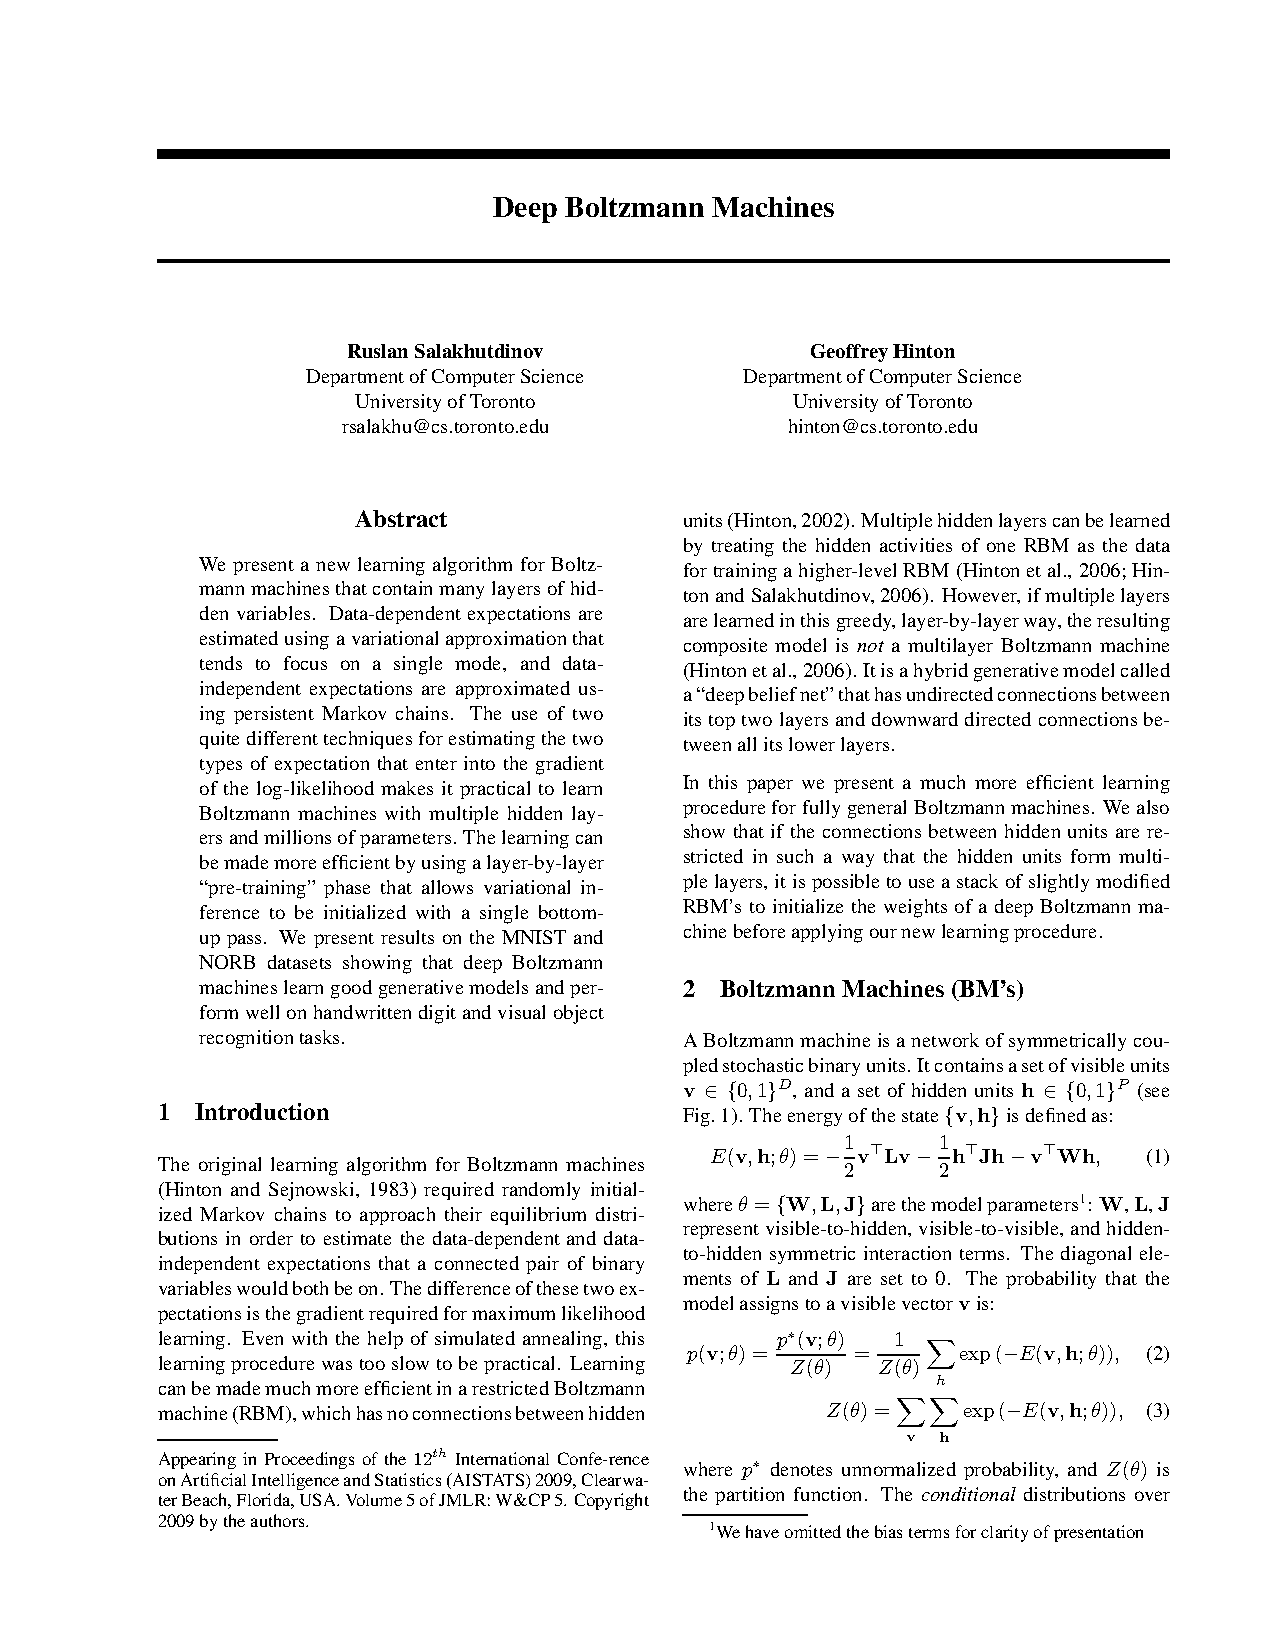
\includegraphics[width = \columnwidth]{../fig/dbm.png}
\caption{(extrême gauche) Un DBN avec sa dernière couche non orientée ; (gauche) graphe de DBM, toutes les couches sont non orientées ; (droite) \emph{pre-training} des RBM couche par couche ; (extrême droite) composition des couches pour former le DBM.}
\label{fig5}
\end{figure}


\end{frame}

\section{debtr}

\end{document}